\documentclass[12pt, letterpaper, oneside]{article}
\usepackage[letterpaper,  left=30mm, right = 30mm, top=45mm, bottom=20mm]{geometry}                		
\usepackage{tikz}
\usepackage{amsmath,amssymb,amscd,amsthm,eucal,curves,epic, graphicx}
\usepackage{enumitem}

%---------------------------------------------------
% TiKZ
%---------------------------------------------------
\newcommand{\btikz}[1][]{\begin{equation*}\begin{tikzpicture}[#1]}
\newcommand{\etikz}{\end{tikzpicture}\end{equation*}}

%---------------------------------------------------
% Fonts
%---------------------------------------------------
\usepackage{pifont}
\usepackage[math]{iwona}

\newcount\problemCount %% problem counter
\problemCount=1
\newcount\subproblemCount %% subproblem counter
\subproblemCount=97 %% 97 = the ascii character code for 'a'


%% \prob resets \subprobCount, typesets problem number according to 
%% \probCounter value and advances \probCounter. 
\newcommand{\prob}[1][]{\subproblemCount=97\noindent{\bf {\number\problemCount}. {{\bf #1}} }\advance\problemCount by 1}


%% \subprobCount typesets subproblem number according to 
%% \subprobCounter value and advances \subprobCount
\newcommand{\subprob}{\par\vskip.2cm\noindent{\bf\char\subproblemCount ) }\advance\subproblemCount by 1}

%% \subprobns is a variant of \subprob which does not skip 
%% vertical space before typesetting the subproblem number.
\newcommand{\subprobns}{\noindent{\bf\char\subproblemCount ) }\advance\subproblemCount by 1}


%%%%%%%%%%%%%%%%%%%%%%%%%%%%
%   END MACROS
%%%%%%%%%%%%%%%%%%%%%%%%%%%%


\begin{document} 

\pagestyle{empty}

%---------------------------------------------------
%  TITLE PAGE
%---------------------------------------------------
\def\pnum{7} % number of problems

\thispagestyle{empty}
\newgeometry{left=10mm, right=10mm, top=40mm, bottom=20mm} 



\begin{center}
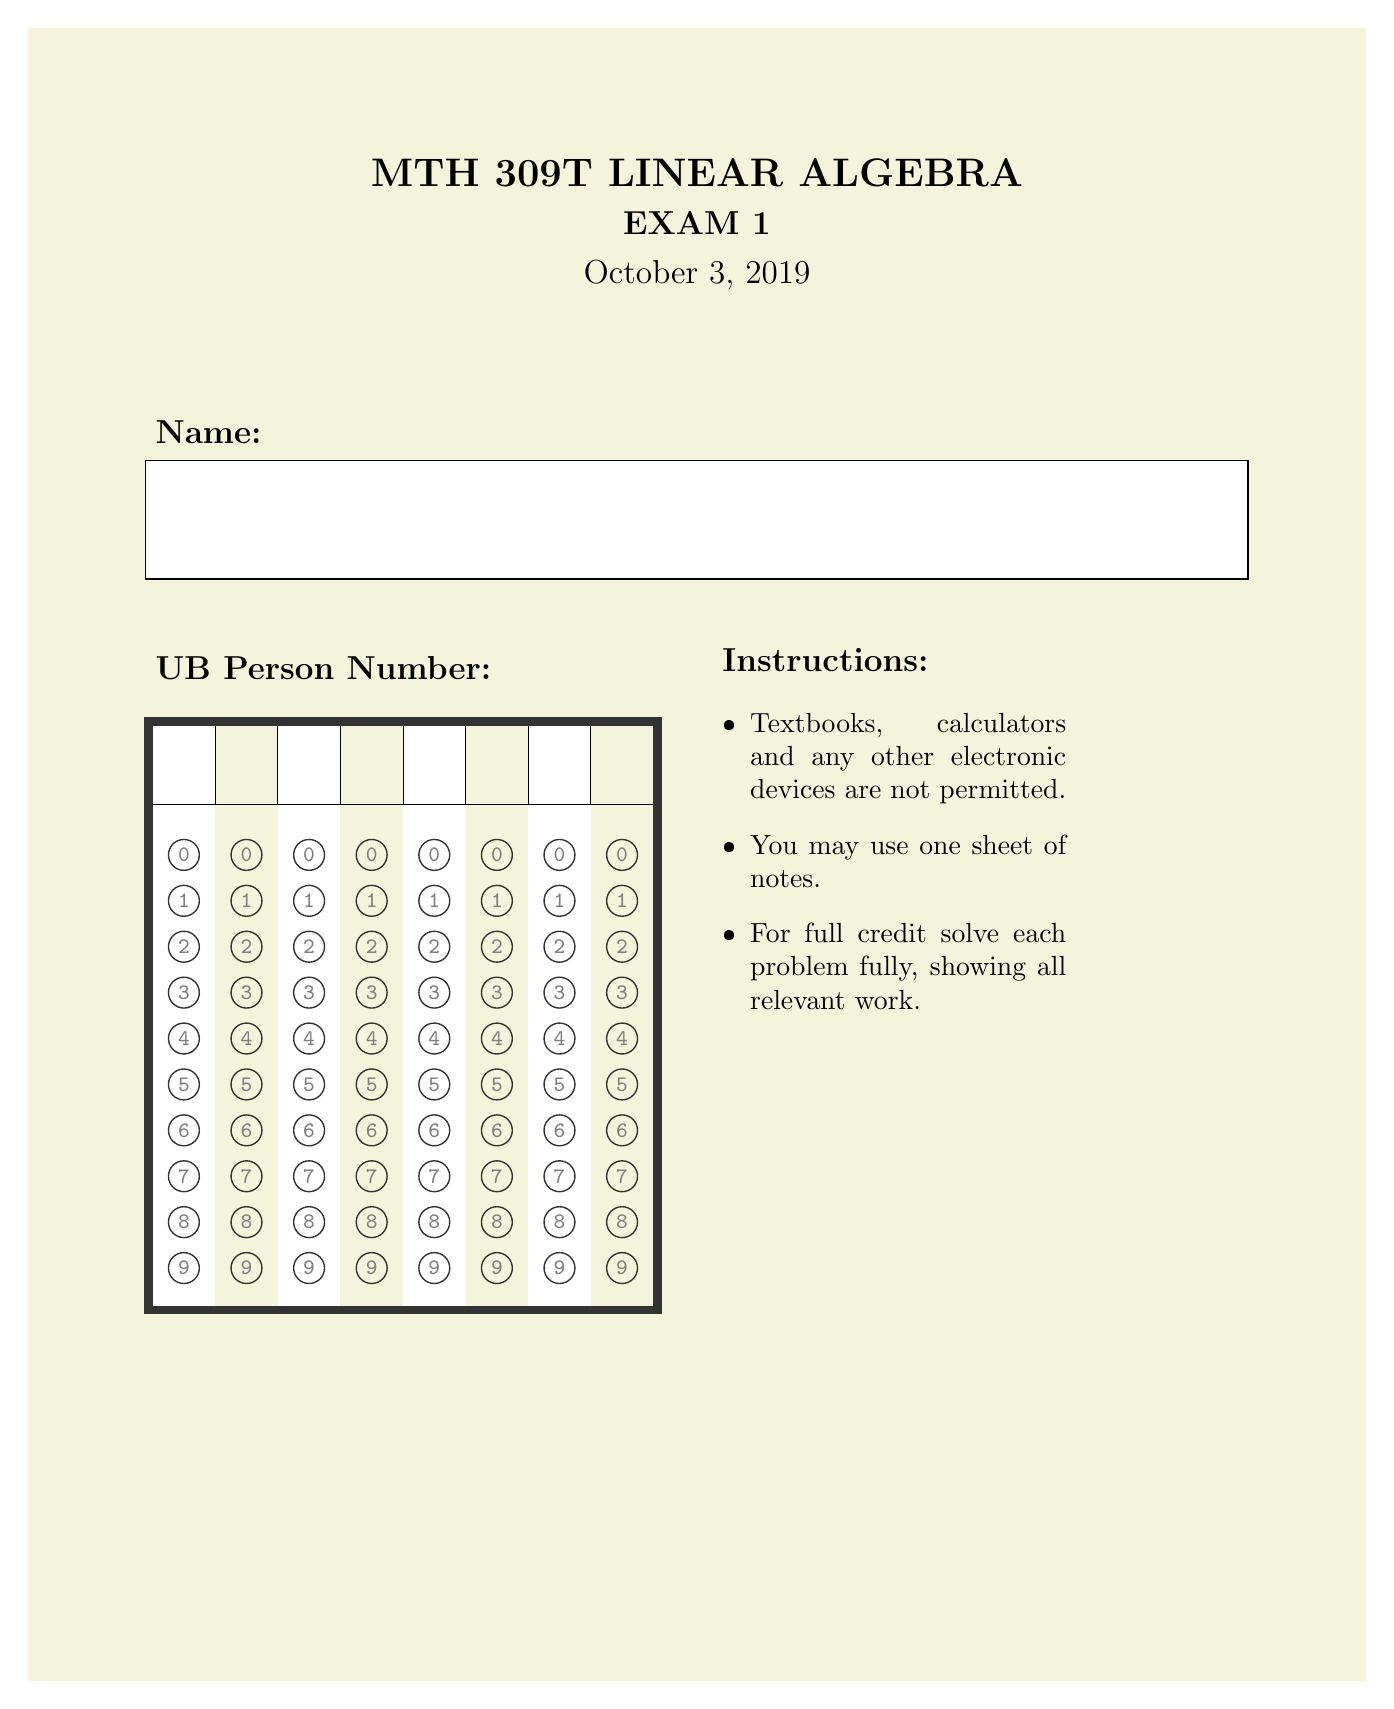
\begin{tikzpicture}
%background and header
\fill[olive!10] (-0.5,0) rectangle (16.5, 21);
\node at (8, 18.5) {\begin{minipage}{\textwidth}
\begin{center}
{\Large \bf{MTH 309T LINEAR ALGEBRA}}\\[2mm]
{\large \bf{EXAM 1}} \\[2mm]
 {\large October 3, 2019} \\
\end{center}
\end{minipage}
};

% name box
\node[anchor = south west] at (1, 15.6) {\large \bf Name:};
\draw[fill  = white, line width = 0.5]  (1, 14) rectangle +(14, 1.5);


% person number
\node[anchor = south west] at (1, 12.6) {\large \bf UB Person Number:};

\begin{scope}[scale=0.53, yshift = 200mm, xshift =13mm]
\draw[black!50, fill = white, line width = 3]  (0.65, 3) rectangle +(8*1.5 + 0.2, -1.1*11-2);

\foreach \x in {1,3,5,7}{
\fill[olive!10]  (0.75 + 1.5*\x, 3) rectangle +(1.5, -1.1*11 - 2);
};
\foreach \x in {1,...,8}{
\draw[line width = 0.3]  (1.5*\x-0.75, 1) rectangle +(1.5, 2);
}

\draw[black!80,  line width = 3]  (0.65, 3) rectangle +(8*1.5 + 0.2, -1.1*11-2);

\foreach \y [evaluate={\z=int(-1*\y);}] in {0,-1,...,-9}{
\foreach \x in {1,...,8}{
\draw[line width = 0.5, color=black!80 ] (1.5*\x, 1.1*\y- 0.2) circle (0.37);
\node at (1.5*\x, 1.1*\y - 0.2) {\footnotesize \color{black!50}\tt \z};
};
}
\end{scope}



% instructions
\node[anchor=north west] at (8.2, 13.24) {\begin{minipage}{0.36\textwidth}
{\large \bf Instructions:}


\begin{itemize}[leftmargin=*]

\item Textbooks, calculators and any other electronic devices are not permitted. 

\item You may use one sheet of notes.  

\item For full credit solve each problem fully, showing all relevant work.
\end{itemize}  

\end{minipage}
};


\end{tikzpicture}
\end{center}

\newpage

\restoregeometry

%---------------------------------------------------
% END TITLE PAGE
%---------------------------------------------------



%---------------------------------------------------
% PROBLEM 1
%---------------------------------------------------


\prob[(20 points)]  This an exam problem. 

\subprob First subproblem. 

\subprob Second subproblem


\newpage 

%---------------------------------------------------
% PROBLEM 2
%---------------------------------------------------


\prob[(10 points)]  \subprobns Subproblem without a new paragraph. 


\subprob Second subproblem. 


\newpage 

%---------------------------------------------------
% PROBLEM 3
%---------------------------------------------------


\prob[(10 points)] 



\end{document}

